\section{Quadriche}

%\begin{tikzpicture}
%	\pgfplotsset{ticks=none}
%    \begin{axis}[
%            xmin=-3,xmax=3,
%            ymin=-3,ymax=3,
%            zmin=-2,zmax=2,
%            xlabel={$x$},
%            ylabel={$y$},
%            zlabel={$z$},
%            zlabel style={rotate=90},
%            view={10}{20},
%            width=3cm,
%            height=3cm]
%        \addplot3[mesh,black,domain=0:2*pi,y domain=0:pi,samples=10,samples y=10]({2*cos(deg(x))*sin(deg(y))},{sin(deg(x))*sin(deg(y))},{cos(deg(y))});
%    \end{axis}
%    
%	\node[text width=1.7cm] at (0.5,-0.4) {$\scriptstyle \frac{x^2}{4}+y^2+z^2=1$};
%\end{tikzpicture}
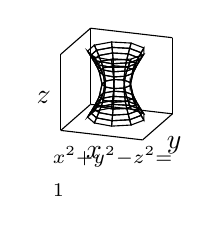
\begin{tikzpicture}
	\pgfplotsset{ticks=none}
    \begin{axis}[
            xmin=-3,xmax=3,
            ymin=-3,ymax=3,
            zmin=-2,zmax=2,
            xlabel={$x$},
            ylabel={$y$},
            zlabel={$z$},
            zlabel style={rotate=90},
            view={20}{20},
            width=3cm,
            height=3cm]
        % x^2+y^2-z^2=1
        \addplot3[mesh,black,domain=1:2,y domain=0:2*pi,samples=6,samples y=10]({x*cos(deg(y))},{x*sin(deg(y))},{sqrt(x^2-1)});
        \addplot3[mesh,black,domain=1:2,y domain=0:2*pi,samples=6,samples y=10]({x*cos(deg(y))},{x*sin(deg(y))},{-sqrt(x^2-1)});
    \end{axis}
    
    \node[text width=1.6cm] at (0.7,-0.4) {$\scriptstyle x^2+y^2-z^2=1$};
\end{tikzpicture}
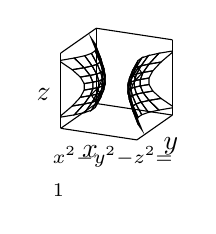
\begin{tikzpicture}
	\pgfplotsset{ticks=none}
    \begin{axis}[
            xmin=-3,xmax=3,
            ymin=-3,ymax=3,
            zmin=-2,zmax=2,
            xlabel={$x$},
            ylabel={$y$},
            zlabel={$z$},
            zlabel style={rotate=90},
            view={25}{20},
            width=3cm,
            height=3cm]
        % x^2-y^2-z^2=1
        \addplot3[mesh,black,domain=-1.2:1.2,y domain=-1.2:1.2,samples=8,samples y=8]({cosh(x)*cosh(y)},{cosh(x)*sinh(y)},{sinh(x)});
        \addplot3[mesh,black,domain=-1.2:1.2,y domain=-1.2:1.2,samples=8,samples y=8]({-cosh(x)*cosh(y)},{cosh(x)*sinh(y)},{sinh(x)});
        
    \end{axis}
    
    \node[text width=1.6cm] at (0.7,-0.4) {$\scriptstyle x^2-y^2-z^2=1$};
\end{tikzpicture}
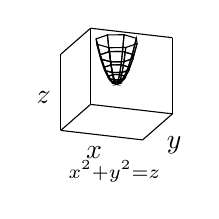
\begin{tikzpicture}
	\pgfplotsset{ticks=none}
    \begin{axis}[
            xmin=-3,xmax=3,
            ymin=-3,ymax=3,
            zmin=-2,zmax=2,
            xlabel={$x$},
            ylabel={$y$},
            zlabel={$z$},
            zlabel style={rotate=90},
            view={20}{20},
            width=3cm,
            height=3cm]
        \addplot3[mesh,black,domain=0:2*pi,y domain=0:1.5,samples=9,samples y=6]({y*cos(deg(x))},{y*sin(deg(x))},{y^2});
        
    \end{axis}
    
    \node[text width=1.2cm] at (0.7,-0.4) {$\scriptstyle x^2+y^2=z$};
\end{tikzpicture}
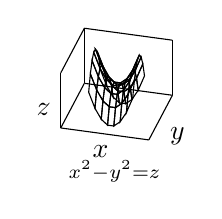
\begin{tikzpicture}
	\pgfplotsset{ticks=none}
    \begin{axis}[
            xmin=-3,xmax=3,
            ymin=-3,ymax=3,
            zmin=-2,zmax=2,
            xlabel={$x$},
            ylabel={$y$},
            zlabel={$z$},
            zlabel style={rotate=90},
            view={15}{40},
            width=3cm,
            height=3cm]
        \addplot3[mesh,black,domain=-1.5:1.5,y domain=-1.5:1.5,samples=8,samples y=8]({x},{y},{x^2-y^2});
        
    \end{axis}
    
    \node[text width=1.2cm] at (0.7,-0.4) {$\scriptstyle x^2-y^2=z$};
\end{tikzpicture}


\textbf{Sfera}: luogo dei punti dello spazio equidistanti da un punto fisso (centro). $x^2+y^2+z^2=r^2$

\textbf{Cono}: luogo di rette per un punto fisso (vertice, centro).

\textbf{Cilindro}: luogo di rette parallele.

Non tutti i coni/cilindri sono quadriche.

\textbf{Rotazioni}: ($z = 0$) $F(x, y)$ attorno $x$ diventa $F(x, \sqrt{y^2+z^2})$
$F(x,y,z)$ è di rotazione $\Leftrightarrow$ ha 2 autoval uguali, diversi da 0.

\begin{tabular}{cccl}
	\textbf{Equazione} & \textbf{Asse} & \textbf{Risultato} & \textbf{Nome} \\
	\hline
	$\frac{x^2}{a^2}+\frac{y^2}{b^2}=1$ & $x$ & $\frac{x^2}{a^2}+\frac{y^2+z^2}{b^2}=1$ & Ellis. di rot. \\
	$\frac{x^2}{a^2}-\frac{y^2}{b^2}=1$ & $x$ & $\frac{x^2}{a^2}-\frac{y^2+z^2}{b^2}=1$ & Iperb. ellit. \\
	$\frac{x^2}{a^2}-\frac{y^2}{b^2}=1$ & $y$ & $\frac{x^2+z^2}{a^2}-\frac{y^2}{b^2}=1$ & Iperb. iperb. \\
	$x^2=2py$ & $x$ & $x^2+z^2=2py$ & Parab. di rot.
\end{tabular}

\textbf{Fascio di quadriche}: $\lambda F(x, y, z) + \mu G(x, y, z) = 0$

\textbf{Forme canoniche}
\setlength{\tabcolsep}{0.2em}%
\begin{tabular}{llccc}
	\textbf{Equazione} & \textbf{Nome} & \textbf{Pnt.} & \textbf{Rig.} & \textbf{Cent.} \\
	\hline
	$\frac{x^2}{a^2} + \frac{y^2}{b^2} + \frac{z^2}{c^2} = 1$ & Ellissoide & E & No & Si \\
	$\frac{x^2}{a^2} + \frac{y^2}{b^2} - \frac{z^2}{c^2} = 1$ & Iperb. iperb. (1 falda) & I & Si & Si \\
	$\frac{x^2}{a^2} - \frac{y^2}{b^2} - \frac{z^2}{c^2} = 1$ & Iperb. ellitt. (2 falde) & E & No & Si \\
	$\frac{x^2}{a^2} + \frac{y^2}{b^2} = 2pz$ & Parab. ellitt. & E & No & No \\
	$\frac{x^2}{a^2} - \frac{y^2}{b^2} = 2pz$ & Parab. iperb. (sella) & I & Si & No \\
	 & Coni e cilindri & P & Si & \\
\end{tabular}

Quadrica $\cap$ piano tangente $=$ 1 retta (punto parabolico), 2 rette incidenti (punto iperbolico), 1 punto (punto ellittico). 

\textbf{Classificazione}
\begin{tabular}{ll}
	$I_1=\tr A = \lambda_1+\lambda_2+\lambda_3$ & $I_2=\lambda_1\lambda_2+\lambda_1\lambda_3+\lambda_2\lambda_3$ \\
	$I_3 = \det A$ & $I_4 = \det B$
\end{tabular}

{
\begin{threeparttable}
\setlength{\tabcolsep}{0.5em}%
\begin{tabular}{c|c|c|c|l|c|c|l}
	\boldmath$I_4$
	         & \boldmath$I_3$
	                 & \boldmath$I_2$
	                       & \boldmath$I_1$
	                               & \boldmath$\vec{x}^TA\vec{x}$\tnote{†}
	                                          & \boldmath$\rk A$
	                                              & \boldmath$\rk B$
	                                                     & \textbf{Nome} \\
	\hline
	+        & $\pm$ & $+$ & $\pm$ & def.     & 3 & 4    & Ellis. imm. \\
	+        & $\pm$ & $-$\tnote{‡} & $\mp$ & indef.   & 3 & 4    & Iperb. iperb. \\
	+        & 0     &     &       &          & 2 & 4    & Parab. iperb. \\
	\hline
	0        & $\pm$ & $+$ & $\pm$ & def.     & 3 & 3    & Cono imm. \\
	0        & $\pm$ & $-$ & $\mp$ & indef.   & 3 & 3    & Cono reale \\
	0        & 0     & $-$ &       & indef.    & 2 & 3    & Cilindro iperb. \\
	0        & 0     & $+$ &       & semi.   & 2 & 3    & Cilindro ellit. \\
	0        & 0     & 0   &       &          & 1 & 3    & Cilindro parab. \\
	0        & 0     &     &       &          & $\le 2$ & 2    & 2 piani distinti \\
	0        & 0     &     &       &          & 1 & 1    & 2 piani coincid. \\
	\hline
	$-$      & $\pm$ & $+$ & $\pm$ & def.     & 3 & 4    & Elliss. reale \\
	$-$      & $\pm$ & $-$\tnote{‡} & $\mp$ & indef.   & 3 & 4    & Iperb. ellit. \\
	$-$      & 0     &     &       &          & 2 & 4    & Parab. ellit. \\
\end{tabular}
\begin{tablenotes}
	\item[†] $\vec{x}^TA\vec{x}$ i termini di 2\textdegree\ grado, equivalente a valutare $I_1$ e $I_2$
	\item[‡] È suffciente che $I_1I_3 \le 0$ o $I_2 \le 0$
\end{tablenotes}
\end{threeparttable}
}
